\documentclass{beamer}

\title{Group 3: LDPC DRAM Decoder/Encoder}
\author{Tom Wang \\ Natalie Balashov}
% \author{Natalie Balashov\\[10mm]{\small Supervisors: \\ Person One \\ Person Two}}
\date{April 10th, 2024}

\begin{document}

\begin{frame}
    \titlepage
\end{frame}

\begin{frame}{Intro}
    Example of lists with Roman numerals:
    \begin{enumerate}[I]
        \item Point A
        \item Point B
              \begin{enumerate}[i]
                  \item part 1
                  \item part 2
              \end{enumerate}
        \item Point C
        \item Point D
    \end{enumerate}
\end{frame}

\begin{frame}{Using Columns}
    \begin{columns}
        \column{0.5\textwidth}
        column 1 with background info
        \column{0.5\textwidth}
        column 2 with more background info
    \end{columns}
\end{frame}

\begin{frame}{Pictures with text below}
    % \begin{figure}
    %     \includegraphics[scale=0.1]{figures/image_name.png}
    %     \caption{A sample figure}
    % \end{figure}
    Insert explanatory text here.
\end{frame}

\begin{frame}{Pictures with text beside}
    \begin{columns}
        \column{0.5\textwidth}
        column 1 with background info
        \column{0.5\textwidth}
        % \begin{figure}
        %     \includegraphics[scale=0.1]{figures/figure_name.png}
        %     \caption{A sample figure}
        % \end{figure}
    \end{columns}
\end{frame}

\begin{frame}{Lists in Beamer}
    This is an unordered list:
    \begin{itemize}
        \item Item 1
        \item Item 2
        \item Item 3
    \end{itemize}
    and this is an ordered list:
    \begin{enumerate}
        \item Item 1
        \item Item 2
        \item Item 3
    \end{enumerate}
\end{frame}

\begin{frame}{Blocks in Beamer}
    \begin{block}{Standard Block}
        This is a standard block.
    \end{block}
    \begin{alertblock}{Alert Message}
        This block presents alert message.
    \end{alertblock}
    \begin{exampleblock}{An example of typesetting tool}
        Example: MS Word, \LaTeX{}
    \end{exampleblock}
\end{frame}

\begin{frame}{Math Blocks in Beamer}
    \begin{definition}
        A prime number is a number that...
    \end{definition}
    \begin{theorem}[Pythagoras]
        $a^2 + b^2 = c^2$
    \end{theorem}
    \begin{corollary}
        $x + y = y + x  $
    \end{corollary}
    \begin{proof}
        $\omega +\phi = \epsilon$
    \end{proof}
\end{frame}

\begin{frame}[fragile]{Including Code}
    \begin{semiverbatim}
        \\begin\{frame\}
        \\frametitle\{Outline\}
        \\tableofcontents
        \\end\{frame\}
    \end{semiverbatim}
    \begin{semiverbatim}
        int function() \{
        int i = 0;
        return i * i;
        \}
    \end{semiverbatim}
\end{frame}

\begin{frame}{Table example}
    \begin{table}
        \begin{tabular}{l | c | c | c | c }
            Competitor Name & Swim  & Cycle & Run   & Total \\
            \hline \hline
            John T          & 13:04 & 24:15 & 18:34 & 55:53 \\
            Norman P        & 8:00  & 22:45 & 23:02 & 53:47 \\
            Alex K          & 14:00 & 28:00 & n/a   & n/a   \\
            Sarah H         & 9:22  & 21:10 & 24:03 & 54:35
        \end{tabular}
        \caption{Triathlon results}
    \end{table}
\end{frame}

\begin{frame}{Hamming implementation}
    Typical Hamming code implementation uses 64-bit to 72-bit encoding.

    This typical implementation is called \textbf{SECDED} (Single Error Correction,
    Double Error Detection) Hamming code.

    The concept of Hamming code is detecting errors in half of the codewords. And
    then with different combinations of deleting patterns, we can locate a single
    bit.

    \begin{figure}[htbp]
        \centerline{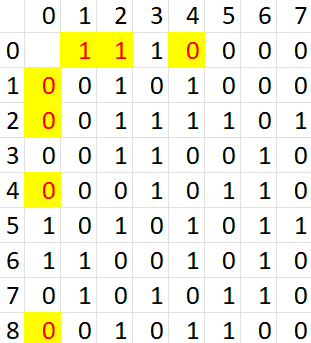
\includegraphics[scale = 0.6]{Images/Hamming_example.png}}
        \caption{Parity bits and data bits in a Hamming code.}
    \end{figure}
\end{frame}

\begin{frame}{Example of correcting error}
    There are a total of 72 bits, which can be expressed in binary from $6'b000\_0000$ to $6'b 100\_0111$.

    Mark the unique position vector as \texttt{vec[6:0]} and let it be bijective to
    parity bits \texttt{p[6:0]}.

    We order the bits as shown below:

    \begin{figure}[htbp]
        \centerline{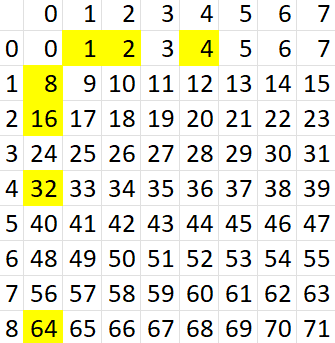
\includegraphics[scale = 0.6]{Images/Hamming_bits_order.png}}
        \caption{Number parity bits and data bits in a Hamming code.}
    \end{figure}
\end{frame}

\begin{frame}{FPGA Implementation}
    Logic can be easily achieved with a series of \textit{xor gates} and \textit{and gates}.

    RTL viewer can be found on GitHub.

    According to Quartus timing analysis, the highest frequency it can run is
    \textbf{387.3 MHz} under \textit{slow 1100 mV 85C mode}.
\end{frame}

\end{document}
